\newpage
%%%%%%%%%%%%%%%%%%%%%%%%%%%%%%%%%%%%%%%%%%%%%%%%%%%%%%%%%%%%%%%%
%%%%%%%%%%%%%%%%%%%%%%%%%%%%%%%%%%%%%%%%%%%%%%%%%%%%%%%%%%%%%%%%
%%%%%%%%%%%%%%%%%%%%%%%%%% Enunciado %%%%%%%%%%%%%%%%%%%%%%%%%%%

\begin{myblock}
\phantomsection\addcontentsline{toc}{section}{Ejercicio \#2 | Modelado de la Probabilidad de Enfermedad Cardíaca según el Nivel de Ronquido}
\section*{Ejercicio \#12| Modelado de la Probabilidad de Enfermedad Cardíaca según el Nivel de Ronquido}

Se tiene la siguiente tabla donde se eligen varios niveles de ronquidos y se ponen en relación con 
una enfermedad cardíaca. Se toman como puntuaciones relativas de ronquidos los valores $\{0, 2, 4, 5\}$.
\\

\begin{tabular}{lccc}
\hline
                & \multicolumn{2}{c}{\textbf{Enfermedad Cardiaca}} &                     \\ \cline{2-3}
\textbf{Ronquido}        & \textbf{SI}            & \textbf{NO}             & \textbf{Proporción de SI} \\ \hline
Nunca           & 24           & 1355          & 0.017               \\
Ocasional       & 35           & 603           & 0.055               \\
Casi cada noche & 21           & 192           & 0.099               \\
Cada noche      & 30           & 224           & 0.118               \\ \hline
\end{tabular}\\

Ajuste un modelo lineal generalizado logit y probit (investigar sobre el link probit), para analizar 
si existe una relación entre los roqnuidos y la posibilidad de tener enfermedad cardiaca. 

\end{myblock}

%%%%%%%%%%%%%%%%%%%%%%%%%%%%%%%%%%%%%%%%%%%%%%%%%%%%%%%%%%%%%%%%
%%%%%%%%%%%%%%%%%%%%%%%%%%%%%%%%%%%%%%%%%%%%%%%%%%%%%%%%%%%%%%%%

\subsection{Teoría}

Lo que queremos hacer en este problema es modelar la probabilidad de una enfermedad cardiaca en función 
del nivel de ronquidos $x_i$, definidos de manera ordinal: $\{0,2,4,5\}$. La probabilidad se modela como
$p_i = Pr(Y=1 | x_i)$. Como nuestra respuesta es binaria, i.e. tenemos conteos de éxito o fracaso por 
categoría, usaremos un GLM binomial con un enlace que mapea de (0,1) a $\mathbb{R}$. De ese modo 
podremmos comparar los dos enlaces estándar: logit y probit. 

Tenemos nuestros datos agrupados entre ``sí'' y ``no''. Para cada fila $i$, tenemos:

\[
    Y_i \sim \text{Binomial}(n_i, p_i) \;\;\;\;\;\; \text{con} \;\; y_i = \text{sí} \;\; \& \;\; n_i - y_i = \text{no}
\]

Por lo que nuestro modelo lineal generalizado queda como:

\[
    g(p_i) = \eta_i = \beta_0 + \beta_1 x_i
\]

Donde $g(\cdot)$ es el enlace. Por lo tanto, para la parte del logit, tenemos:

\[
    g(p) = \text{logit}(p) = \text{log}(\frac{p}{1-p})
\]

Entonces:

\[
    \text{log}(\frac{p}{1-p}) = \beta_0 + \beta_1 x_i \;\;\;\;\; => \;\;\;\;\; p_i = \frac{\text{exp}(\beta_0 + \beta_1 x_i)}{1 + \text{exp}(\beta_0 + \beta_1 x_i)}
\]

Esto nos está indicando que un cambio en $\Delta x$ multiplica los odds por $\exp(\beta_1 \Delta x)$, y 
en particular el odds ratio por unidad de $x$ es $\exp(\beta_1)$.

Ahora, en cuanto al enlace probit, tenemos:

\[
    g(p) = \phi^{-1}(p)
\]

Donde $\phi$ es la CDF Normal estándar, tal que tenemos un modleo de variable latente:

\[
    Z_i = \beta_0 + \beta_1 x_i + \epsilon_i \;\;\;\;\; \epsilon_i \sim \mathcal{N}(0,1) \;\;\;\;\; Y_i = 1\{Z_i > 0\} \;\; => \;\; p_i = \phi(\beta_0+\beta_1 + x_i)
\]

Entonces, para datos agrupados, tenemos una estimación de la log-verosimilitud de la forma:

\[
    \ell(\beta) = \sum_{i} \big[ y_i \text{log}(p_i) + (n_i - y_i) \text{log}(1-p_i) \big]
\]

Con $p_i$ como función de $\eta_i$ via el enlace. Así, se maximiza y los errores estándar provienen
de l amatriz de información observada. 

Además, tanto logit como probit producen curvas sigmoides muy similares. Las pendientes de ambas se
relacionan aproximadamente por un factor de escala:

\[
    \beta_{\text{logit}} \approx 1.7 \times \beta_{\text{probit}}
\]

De este modo, el modleo lineal generalizado aprende d euna sigmoide $p(x)$ que crece si $\beta_1 > 0$, 
i.e. con el nivel de ronquidos. 


%%%%%%%%%%%%%%%%%%%%%%%%%%%%%%%%%%%%%%%%%%%%%%%%%%%%%%%%%%%%%%%%%%%%%%%%%%%%
%%%%%%%%%%%%%%%%%%%%%%%%%%%%%%%%%%%%%%%%%%%%%%%%%%%%%%%%%%%%%%%%%%%%%%%%%%%%

\subsection{Resultados}

Tras ajustar los modelos de GLM binomiales a nuestros datos agrupados, los casos negativos o positivos
de enfermedad cardíaca por nivel de ronquidos, se compararon os enlaces logit y probit mediante AIC y 
deviance. Podemos visualizar el resultado en la figura \ref{fig:logit-probit-02}, mostrada a continuación.

\begin{figure}[h!]
    \centering
    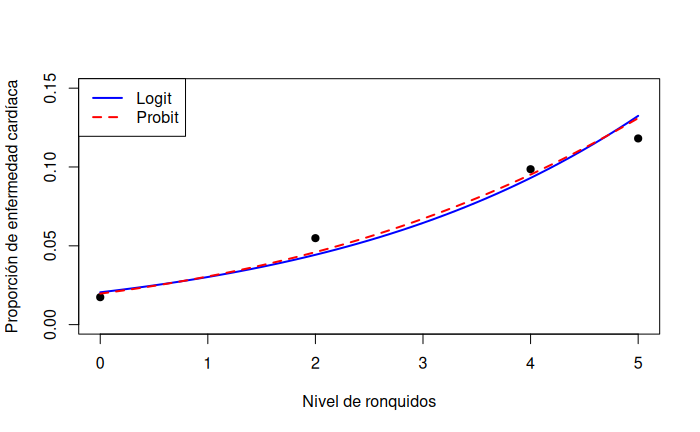
\includegraphics[width=0.7\linewidth]{Images/logit-probit-p02.png}
    \caption{Modelo logit vs. probit.}
    \label{fig:logit-probit-02}
\end{figure}

El cálculo propuesto encontró una asociación positiva y altamente significativa entre ronquidos y enfermedades
cardíacas con un $p-value < 10^{-6}$. En el modelo logit, tenemos un coeficiente de pendiente $\hat{\beta}_1 \approx 0.397$.
En cuanto al odds ratio por unidad en nuestra escala de roqnuidos, tenemos un valor de 1.49 con IC95\% $\approx [1.35, 1.64]$. 
Ahora, hablando del modleo probit, tenemos una pendiente de $\hat{\beta}_1 \approx 0.188$. Lo anterior 
confirma quye tenemos una misma tendencia, pues las magnitudes solo difieren un poco en escala. 

La diferencia por comparación de ajustes es $\text{AIC}(\text{logit} = 27.06)$ y $\text{AIC}(\text{probit} = 26.12)$. Tenemos
una discrepancia muy pequeña de apenas $\Delta \text{AIC} \approx 0.94$, por lo que ambos modelos se 
pueden considerar como equivalentes. 

La probabilidades predichas siguen de cerca las proporciones observadas, con subestimación leve en 
el nivel de roqnuidos 2 y sobreestimación ligera en el nivel 5. Además, un incremento de una unidad
en la escala de roqnuidos eleva la probabilidad de enfermedad cardiaca en un rango aproximado de 1.3 a 1.5
puntos porcentuales, dpeendiendo del nivel de referencia. 

De todo lo anterior, podeos llegar a la conclusión de que hay evidencia robusta de que a mayor frecuencia
de ronquidos, mayor es la probabilidad de presentar enfermedades cardíacas. Tanto el modleo logit como 
el modelo probit describen de manera adecuada el patrón de crecimiento, aunque el probit demuestra un ajuste
ligeramente mejor. Sin embargo, la diferencia entre ambos es muy pequeña. Quizás para casos médicos, es 
relevante escoger los modelos con mejor ajuste, aunque sea minimo, debido a la naturaleza del sector 
salud, donde justo la salud de los pacientes está en juego. 

%%%%%%%%%%%%%%%%%%%%%%%%%%%%%%%%%%%%%%%%%%%%%%%%%%%%%%%%%%%%%%%%%%%%%%%%%%%%
%%%%%%%%%%%%%%%%%%%%%%%%%%%%%%%%%%%%%%%%%%%%%%%%%%%%%%%%%%%%%%%%%%%%%%%%%%%%

%\subsection{Conclusiones}

%%%%%%%%%%%%%%%%%%%%%%%%%%%%%%%%%%%%%%%%%%%%%%%%%%%%%%%%%%%%%%%%%%%%%%%%%%%%
%%%%%%%%%%%%%%%%%%%%%%%%%%%%%%%%%%%%%%%%%%%%%%%%%%%%%%%%%%%%%%%%%%%%%%%%%%%%


\subsection{Código}

\begin{lstlisting}[caption={Modelos Logit y Probit para Enfermedad Cardiaca}, label={lst:glm_r}]
# Carga de datos
ronquidos <- c(0, 2, 4, 5)
si        <- c(24, 35, 21, 30)
no        <- c(1355, 603, 192, 224)
datos     <- data.frame(ronquidos = ronquidos, si = si, no = no)

# Ajuste de modelos GLM
modelo_logit  <- glm(cbind(si, no) ~ ronquidos, family = binomial(link = "logit"), data = datos)
modelo_probit <- glm(cbind(si, no) ~ ronquidos, family = binomial(link = "probit"), data = datos)

# Resumenes y comparacion
summary(modelo_logit)
summary(modelo_probit)
AIC(modelo_logit, modelo_probit)

# Predicciones para graficar
ronq_seq    <- seq(0, 5, by = 0.1)
pred_logit  <- predict(modelo_logit, newdata = data.frame(ronquidos = ronq_seq), type = "response")
pred_probit <- predict(modelo_probit, newdata = data.frame(ronquidos = ronq_seq), type = "response")

# Grafico comparativo
plot(ronquidos, si / (si + no), pch = 19, ylim = c(0, 0.15),
     xlab = "Nivel de ronquidos", ylab = "Proporcion de enfermedad cardiaca")
lines(ronq_seq, pred_logit, col = "blue", lwd = 2)
lines(ronq_seq, pred_probit, col = "red", lwd = 2, lty = 2)
legend("topleft", legend = c("Logit", "Probit"), col = c("blue", "red"), lty = c(1,2))
\end{lstlisting}

\subsection{Resumen de código}

\begin{itemize}
    \item \textbf{Datos:} Se cargan los datos en un \texttt{data.frame} que contiene los conteos de respuestas (\texttt{si}, \texttt{no}) y la variable predictora (\texttt{ronquidos}).

    \item \textbf{Modelos:} Se ajustan modelos lineales generalizados (\texttt{glm}) con la familia \texttt{binomial}, usando \texttt{link = "logit"} para la regresión logística y \texttt{link = "probit"} para el modelo probit. La respuesta se especifica para datos agrupados mediante \texttt{cbind(éxitos, fracasos)}.

    \item \textbf{Análisis:} Se utiliza \texttt{summary()} para obtener estimadores, errores estándar, estadísticos z y valores p. La calidad de ajuste entre modelos se compara con el Criterio de Información de Akaike usando \texttt{AIC()}.

    \item \textbf{Predicciones:} Se calculan las probabilidades predichas por cada modelo sobre una malla de valores de la variable \texttt{ronquidos} para facilitar la visualización.

    \item \textbf{Visualización:} Se genera un gráfico que muestra las proporciones observadas de los datos junto con las curvas de probabilidad predichas por los modelos logit y probit para una comparación visual del ajuste.
\end{itemize}


%%%%%%%%%%%%%%%%%%%%%%%%%%%%%%%%%%%%%%%%%%%%%%%%%%%%%%%%%%%%%%%%%%%%%%%%%%%%
%%%%%%%%%%%%%%%%%%%%%%%%%%%%%%%%%%%%%%%%%%%%%%%%%%%%%%%%%%%%%%%%%%%%%%%%%%%%

\clearpage




















